	%%%%%%%%%%%%%%%%%%%%%%%%%%%%%%%%%%%%%%%%%
% Beamer Presentation
% LaTeX Template
% Version 1.0 (10/11/12)
%
% This template has been downloaded from:
% http://www.LaTeXTemplates.com
%
% License:
% CC BY-NC-SA 3.0 (http://creativecommons.org/licenses/by-nc-sa/3.0/)
%
%%%%%%%%%%%%%%%%%%%%%%%%%%%%%%%%%%%%%%%%%

%----------------------------------------------------------------------------------------
%	PACKAGES AND THEMES
%----------------------------------------------------------------------------------------

\documentclass[usenames,dvipsnames]{beamer}
\usepackage{xcolor}

\mode<presentation> {

% The Beamer class comes with a number of default slide themes
% which change the colors and layouts of slides. Below this is a list
% of all the themes, uncomment each in turn to see what they look like.

%\usetheme{default}
%\usetheme{AnnArbor}
%\usetheme{Antibes}
%\usetheme{Bergen}
%\usetheme{Berkeley}
%\usetheme{Berlin}
%\usetheme{Boadilla}
%\usetheme{CambridgeUS}
%\usetheme{Copenhagen}
%\usetheme{Darmstadt}
%\usetheme{Dresden}
%\usetheme{Frankfurt}
%\usetheme{Goettingen}
%\usetheme{Hannover}
%\usetheme{Ilmenau}
%\usetheme{JuanLesPins}
%\usetheme{Luebeck}
\usetheme{Madrid}
%\usetheme{Malmoe}
%\usetheme{Marburg}
%\usetheme{Montpellier}
%\usetheme{PaloAlto}
%\usetheme{Pittsburgh}
%\usetheme{Rochester}
%\usetheme{Singapore}
%\usetheme{Szeged}
%\usetheme{Warsaw}

% As well as themes, the Beamer class has a number of color themes
% for any slide theme. Uncomment each of these in turn to see how it
% changes the colors of your current slide theme.

%\usecolortheme{albatross}
\usecolortheme{beaver}
%\usecolortheme{beetle}
%\usecolortheme{crane}
%\usecolortheme{dolphin}
%\usecolortheme{dove}
%\usecolortheme{fly}
%\usecolortheme{lily}
%\usecolortheme{orchid}
%\usecolortheme{rose}
%\usecolortheme{seagull}
%\usecolortheme{seahorse}
%\usecolortheme{whale}
%\usecolortheme{wolverine}

%\setbeamertemplate{footline} % To remove the footer line in all slides uncomment this line
%\setbeamertemplate{footline}[page number] % To replace the footer line in all slides with a simple slide count uncomment this line

%\setbeamertemplate{navigation symbols}{} % To remove the navigation symbols from the bottom of all slides uncomment this line
}
\usepackage{tikz}

\usepackage{listings}
\usepackage{graphicx} % Allows including images
\usepackage{booktabs} % Allows the use of \toprule, \midrule and \bottomrule in tables
%\usepackage[T1]{fontenc}
\usepackage[utf8]{inputenc}




%----------------------------------------------------------------------------------------
%	TITLE PAGE
%----------------------------------------------------------------------------------------

\title[LINGI2142 Project 2]{LINGI2142 Computer Networks \\ Project 2} % The short title appears at the bottom of every slide, the full title is only on the title page
\titlegraphic{
\includegraphics[height=2cm]{ingi.png}}

\author[Group 2] {Group 2} % Your name
\institute[INGI] % Your institution as it will appear on the bottom of every slide, may be shorthand to save space
{
Université Catholique de Louvain - INGI\\ % Your institution for the title page
\medskip
}
\date{2nd April 2014} % Date, can be changed to a custom date

%--------------------------------------
% ENVIRONMENT CUSTOMIZED
%--------------------------------------

\newenvironment{blockexample}[1]{
  \setbeamercolor{block title}{bg=OliveGreen}
  \begin{block}{Example : #1}}{\end{block}}


\begin{document}

\begin{frame}
\titlepage % Print the title page as the first slide
\end{frame}

\section{Introduction}
\begin{frame}
\frametitle{Introduction}
\centering 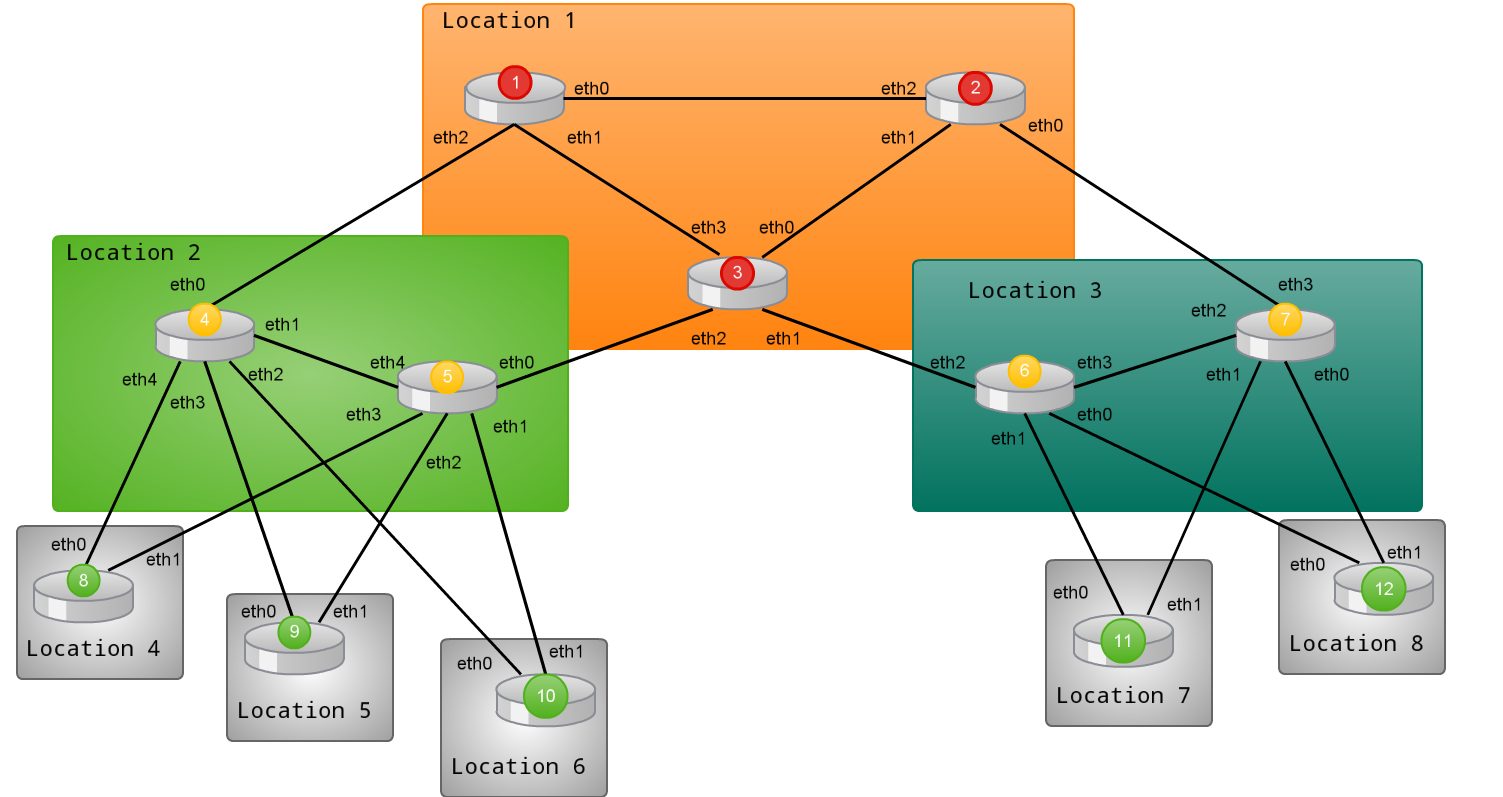
\includegraphics[scale=0.20]{network.png}

\end{frame}

\section{Address Plan}
\begin{frame}
\frametitle{Address Plan}
IPv6 addresses are divided in:
\begin{itemize}
\item \texttt{Prefix} part : $2001:bb8:1234::/48$
\item \texttt{Type part} : $2001:bb8:1234:T:/52$
\item \texttt{Location part} : $2001:bb8:1234:TL:/56$
\end{itemize}
\end{frame}

\begin{frame}
\frametitle{Address Plan : Types}
Different types are defined (16 values available): 
\begin{itemize}
\item \texttt{1}: Infrastructure
\item \texttt{2} : TV - Multicast
\item \texttt{3}: VoIP
\item \texttt{4}: Not Defined yet (free for more VoIP configuration)
\item \texttt{5-8}: Wifi (5 for main, 6 for guests, 7 for external devices, 8 not defined yet but planned for more wifi development)
\item \texttt{9-12}: Services
\item \texttt{13}: Company Ethernet
\item \texttt{14}: Public Ethernet
\item \texttt{15-16}: Not defined yet
\end{itemize}
\end{frame}

\begin{frame}
\frametitle{Bridge}
\begin{blockexample}{Configuration of router 11}
config interface 'eth'\\

\hspace{1cm} option ifname 'eth0 eth1' \\
\hspace{1cm} option type 'bridge' \\
\hspace{1cm}	option stp '1' \\
\hspace{1cm}	option proto 'static' \\
\hspace{1cm} option ip6addr '2001:bb8:1234:3700::11/48' \\
\hspace{1cm} option ip6prefix '2001:bb8:1234::/48' \\
\end{blockexample}

\end{frame}

\begin{frame}
\frametitle{Building addresses}
\centering 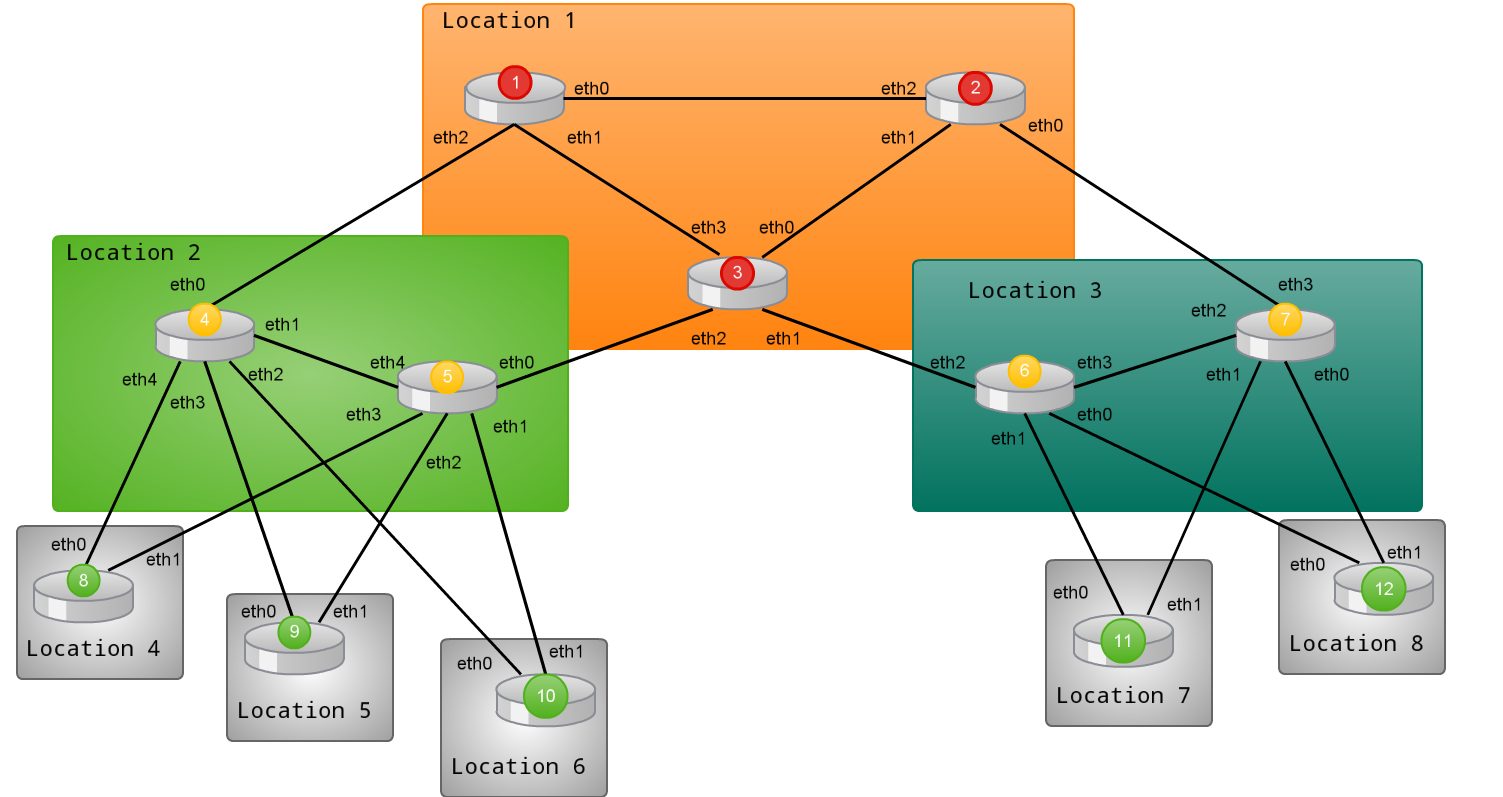
\includegraphics[scale=0.16]{network.png} \\
Addresses : \\

\only<1>{Router 1 : $2001:bb8:1234:1100::1$}
\only<2>{Router 2 : $2001:bb8:1234:1100::2$}
\only<3>{Router 4 : $2001:bb8:1234:1200::4$}
\only<4>{Router 8 : $2001:bb8:1234:2400::8$}
\only<5>{Router 9 : $2001:bb8:1234:3500::9$}

\end{frame}

\section{Security}
\begin{frame}
\frametitle{Security rules}
\begin{itemize}
\item Firewall configuration
\item Iptables rules : ping - ICMP6 rejection
\end{itemize}
\end{frame}

\section{Live Demo}
\begin{frame}
\frametitle{Live Demo}
\begin{Huge}\begin{center}
Live Demo
\end{center}\end{Huge}
\end{frame}


%\section{Issues}
%\begin{frame}
%\frametitle{Issues}
%\begin{columns}[cc]
%\column{.5\textwidth}
%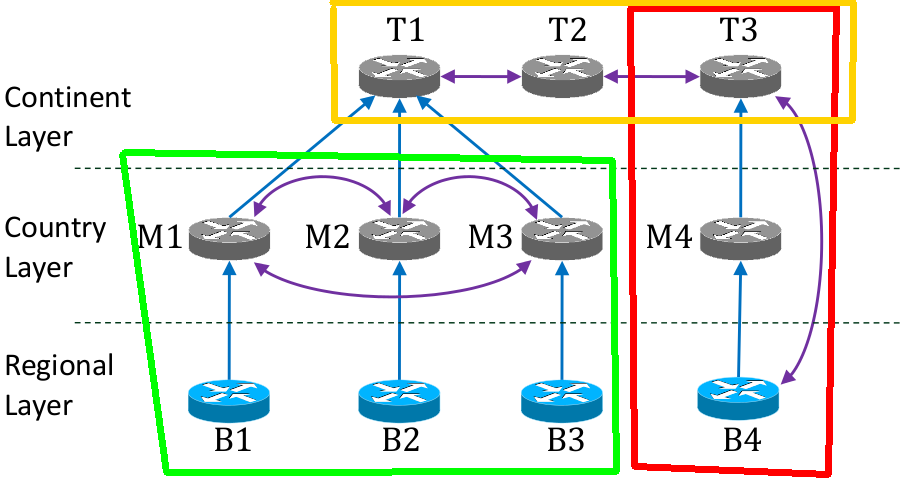
\includegraphics[width=1.3\textwidth]{issues.png}
%\column{.05\textwidth}
%\column{.3\textwidth}
%
%\begin{itemize}
%	\item Peer link between B4 and T3.
%	\item Routes transmission between T1 and T3.
%	\item Oscillation on M1-M2-M3.
%\end{itemize}
%\end{columns}
%\end{frame}
%
%\begin{frame}
%\frametitle{First issue : Peer link between B4 and T3}
%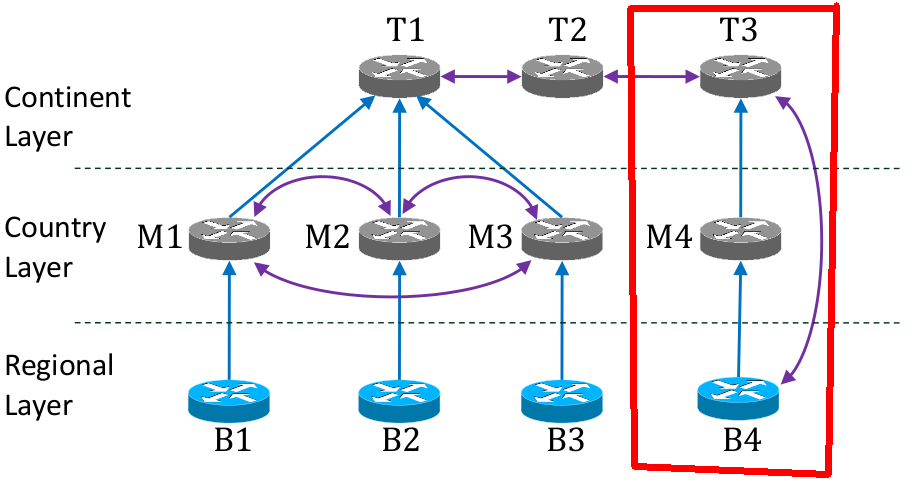
\includegraphics[scale=0.35]{first_issue.png}
%\end{frame}
%
%\begin{frame}
%\frametitle{Solution}
%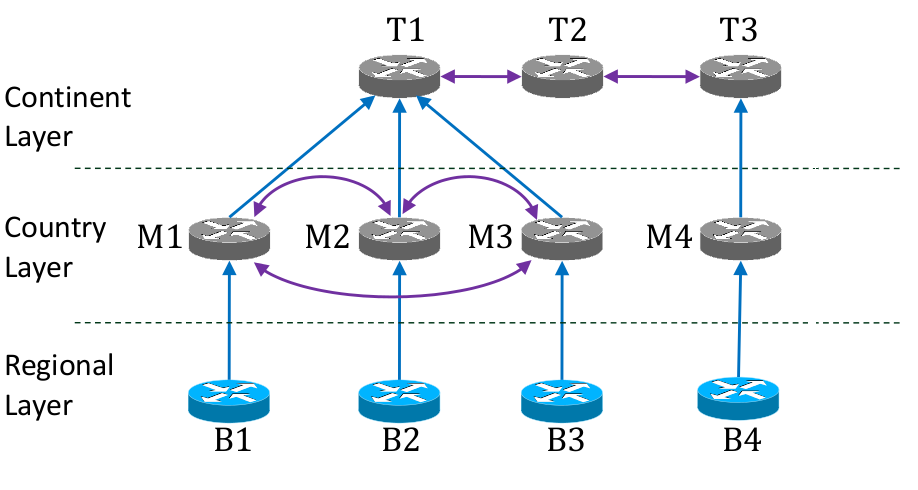
\includegraphics[scale=0.35]{solutions1.png}
%\end{frame}
%
%\begin{frame}
%\frametitle{Second issue : Route transmission between T1 and T3}
%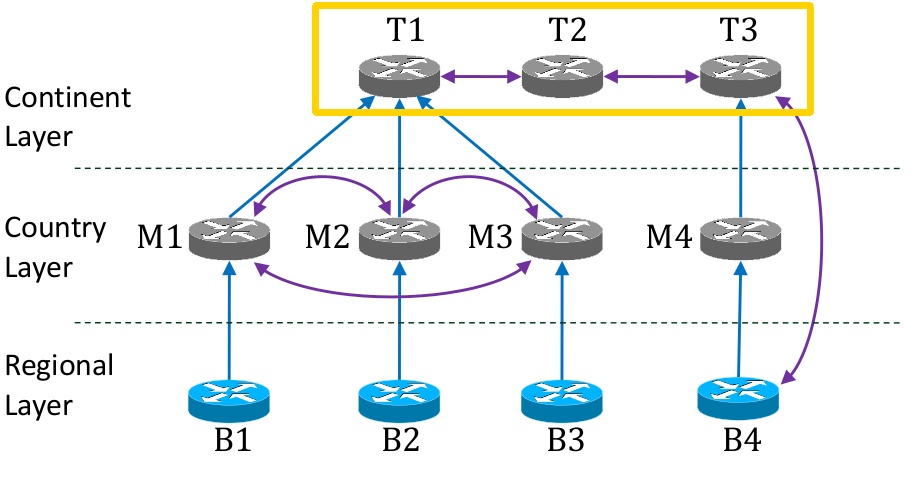
\includegraphics[scale=0.35]{second_issue.png}
%\end{frame}
%
%\begin{frame}
%\frametitle{Solution}
%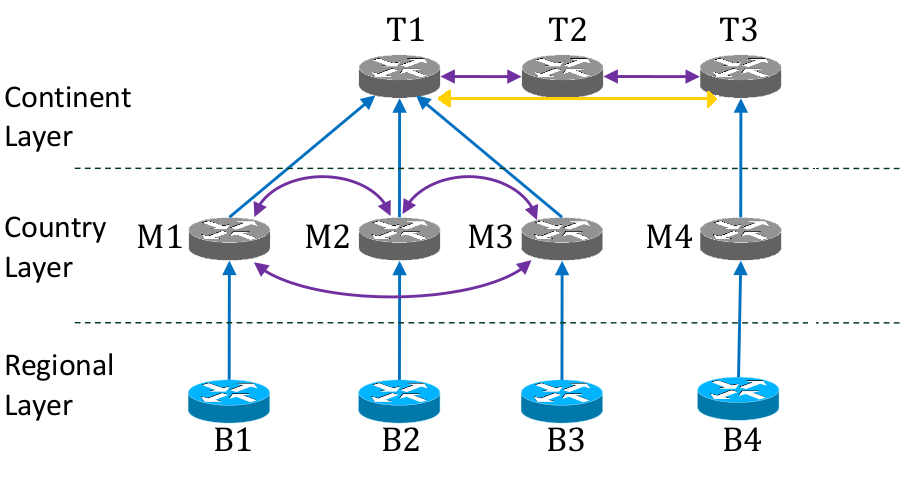
\includegraphics[scale=0.35]{solutions.png}
%\end{frame}
%
%\begin{frame}
%\frametitle{Third issue : Oscillation on M1-M2-M3}
%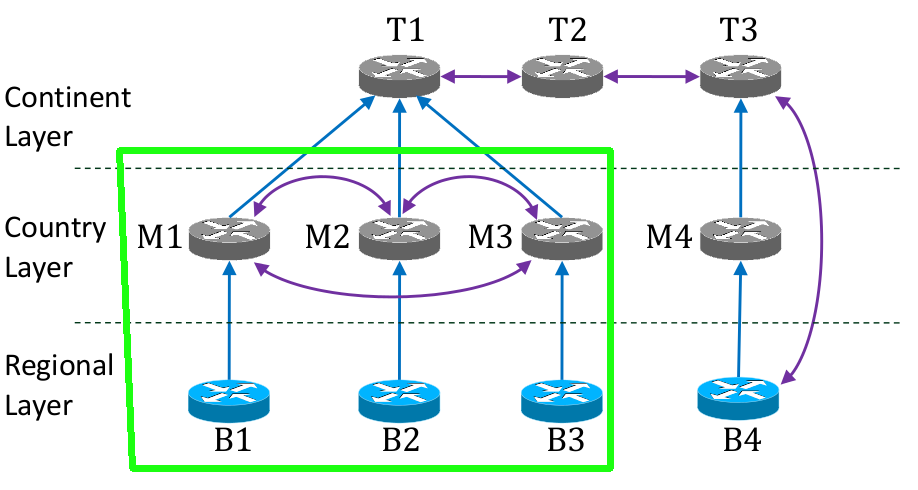
\includegraphics[scale=0.35]{third_issue.png}
%\end{frame}
%
%\begin{frame}
%\frametitle{Solutions}
%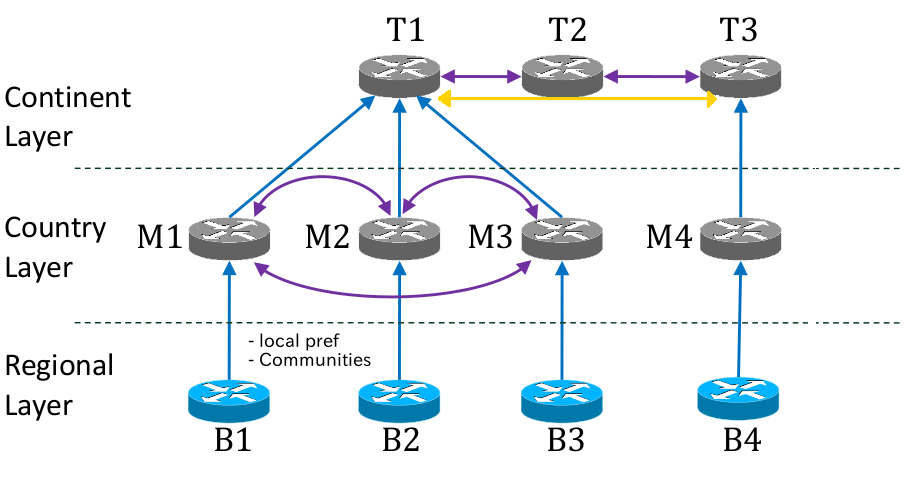
\includegraphics[scale=0.35]{solutions3.png}
%\end{frame}
%
%
%
%%%------------------------------------------------
%%
%%\section{Présentation}
%%
%%\begin{frame}
%%\frametitle{Android}
%%\begin{columns}[c]
%%\column{.4\textwidth}
%%\begin{itemize}
%%\item Système d'exploitation (Comme Windows, MacOs, Ubuntu, ...)
%%\item Open Source
%%\item Dirigé par Google
%%\end{itemize}
%%\column{.3\textwidth}
%%\includegraphics[scale=0.1]{./../Ressources/android.png}
%%\end{columns}
%%\end{frame}
%%
%%\begin{frame}
%%\frametitle{Quelques notions}
%%\begin{block}{Système d'exploitation (\textbf{OS})}
%%\begin{columns}[c]
%%\column{.4\textwidth}
%%\begin{itemize}
%%\item Ensemble de programmes
%%\item Relation hardware - software - utilisateur
%%\end{itemize}
%\column{.4\textwidth}
%\includegraphics[scale=0.2]{./../Ressources/os.png}
%\end{columns}
%\end{block}
%\end{frame}
%
%\begin{frame}
%\frametitle{Quelques notions}
%\begin{block}{Open Source - Logiciel Libre}
%\begin{columns}[c]
%\column{.5\textwidth}
%Possibilités :
%\begin{itemize}
%\item de redistribuer gratuitement
%\item d'accès au code source
%\item de modifier le travail
%\end{itemize}
%Opposition aux logiciels propriétaires\\
%\column{.4\textwidth}
%\includegraphics[scale=0.2]{./../Ressources/opensource.png}\includegraphics[scale=0.12]{./../Ressources/gnu.png}
%\end{columns}
%\end{block}
%\end{frame}
%
%\begin{frame}
%\frametitle{\includegraphics[scale=0.1]{./../Ressources/google.png}}
%\textbf{Moteur de recherche} : application web permettant de trouver des ressources sur le web à travers des mots clés. \\
%Mais aussi :
%\begin{columns}[c]
%\column{.5\textwidth}
%\begin{itemize}
%\item client mail
%\item online storage
%\item calendrier
%\item etc ...
%\end{itemize}
%\column{.4\textwidth}
%\includegraphics[scale=0.2]{./../Ressources/multi.png}
%\end{columns}
%\vspace{0.1in}
%Dans le cadre de ce stage, vous aurez besoin d'un compte Google pour utiliser l'application App Inventor.
%\end{frame}
%
%\begin{frame}
%\frametitle{\includegraphics[scale=0.1]{./../Ressources/appinv.png}}
%\begin{block}{\includegraphics[scale=0.1]{./../Ressources/mit.jpg}}
%\begin{itemize}
%\item Institution de recherche
%\item Université Américaine
%\item Située à Cambridge dans le Massachussets
%\end{itemize}
%\end{block}
%\begin{block}{App Inventor}
%\begin{itemize}
%\item Application web et \textsc{JAVA} permettant de de créer facilement de petites applications pour le système d'exploitation Android.
%\item Pas besoin d'être familier aux langages de programmation
%\item Ludique, intuitif et basé sur une interface graphique où l'on construit l'application comme un puzzle. (basé le système \textsc{Scratch})
%\end{itemize}
%\end{block}
%\end{frame}
%
%\begin{frame}
%\frametitle{\includegraphics[scale=0.1]{./../Ressources/appinv.png}}
%\begin{center}
%\htmladdnormallink{\includegraphics[scale=0.22]{./../Ressources/appdiag.png}}{http://beta.appinventor.mit.edu}
%\end{center}
%\end{frame}
%
%\begin{frame}
%\frametitle{\includegraphics[scale=0.1]{./../Ressources/appinv.png}\ Hello World !}
%\begin{huge}
%Maintenant, à vous de jouer !
%\end{huge}
%\vspace{0.3in}
%\begin{itemize}
%\item Familiarisez vous avec l'interface
%\item Personnalisez ce qui peut l'être
%\item Effectuez le premier test avec la tablette
%\end{itemize}
%\end{frame}
%
%\begin{frame}
%\frametitle{\includegraphics[scale=0.1]{./../Ressources/appinv.png}\ Un peu plus loin...}
%Tout celà est bien statique !\\
%Et si on ajoutait un bonjour un peu plus sonore ?
%\end{frame}
%
%\begin{frame}
%\frametitle{\includegraphics[scale=0.1]{./../Ressources/appinv.png}\ Ce que vous devriez obtenir}
%\begin{block}{Un Hello World très moche}
%
%\end{block}
%\end{frame}
%
%\begin{frame}
%\frametitle{Notions de programmation}
%\begin{itemize}
%\item Variable
%\begin{itemize}
%\item Conteneur
%\item Nom
%\end{itemize}
%\item Type
%\begin{itemize}
%\item Nombre
%\item Texte
%\item Booléen
%\item Objets...
%\end{itemize}
%\end{itemize}
%\begin{blockexemple}{}
%Dans l'App Inventor, vous pouvez créer une variable et y accéder grâce à ces pièces : \\\center\includegraphics[scale=0.2]{./../Ressources/puzzle2.png}
%\end{blockexemple}
%\end{frame}
%
%\begin{frame}
%\frametitle{Notions de programmation - Variables}
%\begin{blockexemple}{Comptage}
%On peut compter le nombre de fois qu'on a appuyé sur un bouton\\
%\begin{center}
%\includegraphics[scale=0.5]{./../Ressources/puzzle4.png}
%\end{center}
%\end{blockexemple}
%
%\end{frame}
%
%
%\begin{frame}
%\frametitle{Notions de programmation - Conditions et boucles}
%\begin{block}{If Then Else}
%\center\color{red} Si \color{black}(condition) \color{red} alors \color{black} \{action\} \color{red} sinon \color{black} \{action\}
%\end{block}
%\begin{blockexemple}{}
%\center\includegraphics[scale=0.5]{./../Ressources/puzzle5.png}
%\end{blockexemple}
%\end{frame}
%
%\begin{frame}
%\frametitle{Notions de programmation - Conditions et boucles}
%\begin{block}{While}
%\center\color{red} Tant que \color{black}(condition) \color{red} alors \color{black} \{action\} 
%\end{block}
%\begin{blockexemple}{}
%\center \includegraphics[scale=0.5]{./../Ressources/puzzle6.png}
%\end{blockexemple}
%\end{frame}

%\begin{frame}
%\frametitle{Blocks of Highlighted Text}
%\begin{block}{Block 1}
%Lorem ipsum dolor sit amet, consectetur adipiscing elit. Integer lectus nisl, ultricies in feugiat rutrum, porttitor sit amet augue. Aliquam ut tortor mauris. Sed volutpat ante purus, quis accumsan dolor.
%\end{block}
%
%\begin{block}{Block 2}
%Pellentesque sed tellus purus. Class aptent taciti sociosqu ad litora torquent per conubia nostra, per inceptos himenaeos. Vestibulum quis magna at risus dictum tempor eu vitae velit.
%\end{block}
%
%\begin{block}{Block 3}
%Suspendisse tincidunt sagittis gravida. Curabitur condimentum, enim sed venenatis rutrum, ipsum neque consectetur orci, sed blandit justo nisi ac lacus.
%\end{block}
%\end{frame}
%
%%------------------------------------------------
%
%\begin{frame}
%\frametitle{Multiple Columns}
%\begin{columns}[c] % The "c" option specifies centered vertical alignment while the "t" option is used for top vertical alignment
%
%\column{.45\textwidth} % Left column and width
%\textbf{Heading}
%\begin{enumerate}
%\item Statement
%\item Explanation
%\item blockexemple
%\end{enumerate}
%
%\column{.5\textwidth} % Right column and width
%Lorem ipsum dolor sit amet, consectetur adipiscing elit. Integer lectus nisl, ultricies in feugiat rutrum, porttitor sit amet augue. Aliquam ut tortor mauris. Sed volutpat ante purus, quis accumsan dolor.
%
%\end{columns}
%\end{frame}
%
%%------------------------------------------------
%\section{Second Section}
%%------------------------------------------------
%
%\begin{frame}
%\frametitle{Table}
%\begin{table}
%\begin{tabular}{l l l}
%\toprule
%\textbf{Treatments} & \textbf{Response 1} & \textbf{Response 2}\\
%\midrule
%Treatment 1 & 0.0003262 & 0.562 \\
%Treatment 2 & 0.0015681 & 0.910 \\
%Treatment 3 & 0.0009271 & 0.296 \\
%\bottomrule
%\end{tabular}
%\caption{Table caption}
%\end{table}
%\end{frame}
%
%%------------------------------------------------
%
%\begin{frame}
%\frametitle{Theorem}
%\begin{theorem}[Mass--energy equivalence]
%$E = mc^2$
%\end{theorem}
%\end{frame}
%
%
%%------------------------------------------------
%
%\begin{frame}
%\frametitle{Figure}
%Uncomment the code on this slide to include your own image from the same directory as the template .TeX file.
%%\begin{figure}
%%\includegraphics[width=0.8\linewidth]{test}
%%\end{figure}
%\end{frame}
%
%
%%------------------------------------------------
%
%\begin{frame}
%\Huge{\centerline{The End}}
%\end{frame}
%
%%----------------------------------------------------------------------------------------
%
\end{document}
